\documentclass[12pt,xcolor=dvipsnames,professionalfonts]{beamer}

% Pakete
\usepackage[utf8]{inputenc}
\usepackage[ngerman]{babel}

% AMS Pakete
\usepackage{amsmath}
\usepackage{amsfonts}
\usepackage{amssymb}

\usepackage{multirow}
\usepackage[percent]{overpic}

% Einheiten
\usepackage{siunitx}
\sisetup{
	output-decimal-marker={,},
	separate-uncertainty
}

% Grafiken
\usepackage{graphicx}
\usepackage{tabularx}
\setbeamerfont{caption}{size=\footnotesize}
\setbeamertemplate{caption}{\raggedright\insertcaption\par}

\newcommand{\todo}[1]{{\textcolor{Green}{(#1)}}}

% Theme
\usetheme{Boadilla}
\usecolortheme{rose}
\useoutertheme{infolines}
\useinnertheme{rectangles}
\setbeamertemplate{itemize subitem}[triangle]

\usefonttheme[onlymath]{serif}

% [num] Zitationen
\setbeamertemplate{bibliography item}[text]

% Navigationsleiste ausschalten
\beamertemplatenavigationsymbolsempty

\DeclareMathOperator{\divergence}{div}

\author[Christopher Deutsch]
{Christopher Deutsch}

\title
{Störkörpermessung an Hohlraumresonatoren}

\subtitle
{}
%\logo{}

\institute[]
{Rheinische Friedrich-Wilhelms-Universität Bonn \\
Seminar zur Bachelorarbeit SS15}

\date{24. September 2015}

%\setbeamercovered{transparent}
%\setbeamertemplate{navigation symbols}{}

\newcommand{\beginbackup}{
	\newcounter{framenumbervorappendix}
	\setcounter{framenumbervorappendix}{\value{framenumber}}
}
\newcommand{\backupend}{
	\addtocounter{framenumbervorappendix}{-\value{framenumber}}
	\addtocounter{framenumber}{\value{framenumbervorappendix}} 
}

\begin{document}
\maketitle

\begin{frame}{Inhalt}
	\tableofcontents
\end{frame}

\section{Motivation}
%\frame{\tableofcontents[currentsection]} Inhaltsverzeichnis für die aktuelle Section
% \setlength\itemsep{1em} in itemization zur abstandeinstellung
\begin{frame}{Motivation (Zuviel Text)}
	\begin{itemize}
		\item Begrenzung des internen Strahlstroms an ELSA durch fehlende Hochfrequenzleistung
		\begin{itemize}
			\setlength\itemsep{0.25em}
			\item max.\ interner Strahlstrom  $\sim\SI{20}{mA}$ bei \SI{3.2}{GeV}
		\end{itemize}
		\vfill
		
		\item Erweiterung des Stretcherrings durch zweite HF-Station
		\begin{itemize}
			\setlength\itemsep{0.25em}
			\item Klystron und zwei 7-zellige PETRA-Resonatoren
			\item interne Strahlströme bis zu \SI{200}{mA}
		\end{itemize}
		\vfill
		
		\item Bestimmung der elektrischen Feldverteilung durch resonante Störkörpermessung
		\begin{itemize}
			\setlength\itemsep{0.25em}
			\item Beschleunigungsspannung
			\item Beschleunigungseffizienz (Shuntimpedanz)
			\item Moden höherer Ordnung
		\end{itemize}
	\end{itemize}
\end{frame}


\section{Hohlraumresonatoren}

\subsection{Schwingungsmoden}
\begin{frame}{Schwingungsmoden}
	\begin{columns}[T]
		\column{0.60\textwidth}
		\begin{itemize}
			\item Hohlraum mit leitenden Wänden
			\begin{itemize}
				\setlength\itemsep{0.25em}
				
				\item stehende em.\ Wellen
				
				\item Randbedingungen:
				\begin{align*}
				E_\parallel = 0 \qquad B_\perp = 0
				\end{align*}
				
				\item erlauben nur bestimmte Feldkonfigurationen (Moden)
			\end{itemize}
		\end{itemize}
		\column{0.4\textwidth}
		\centering
		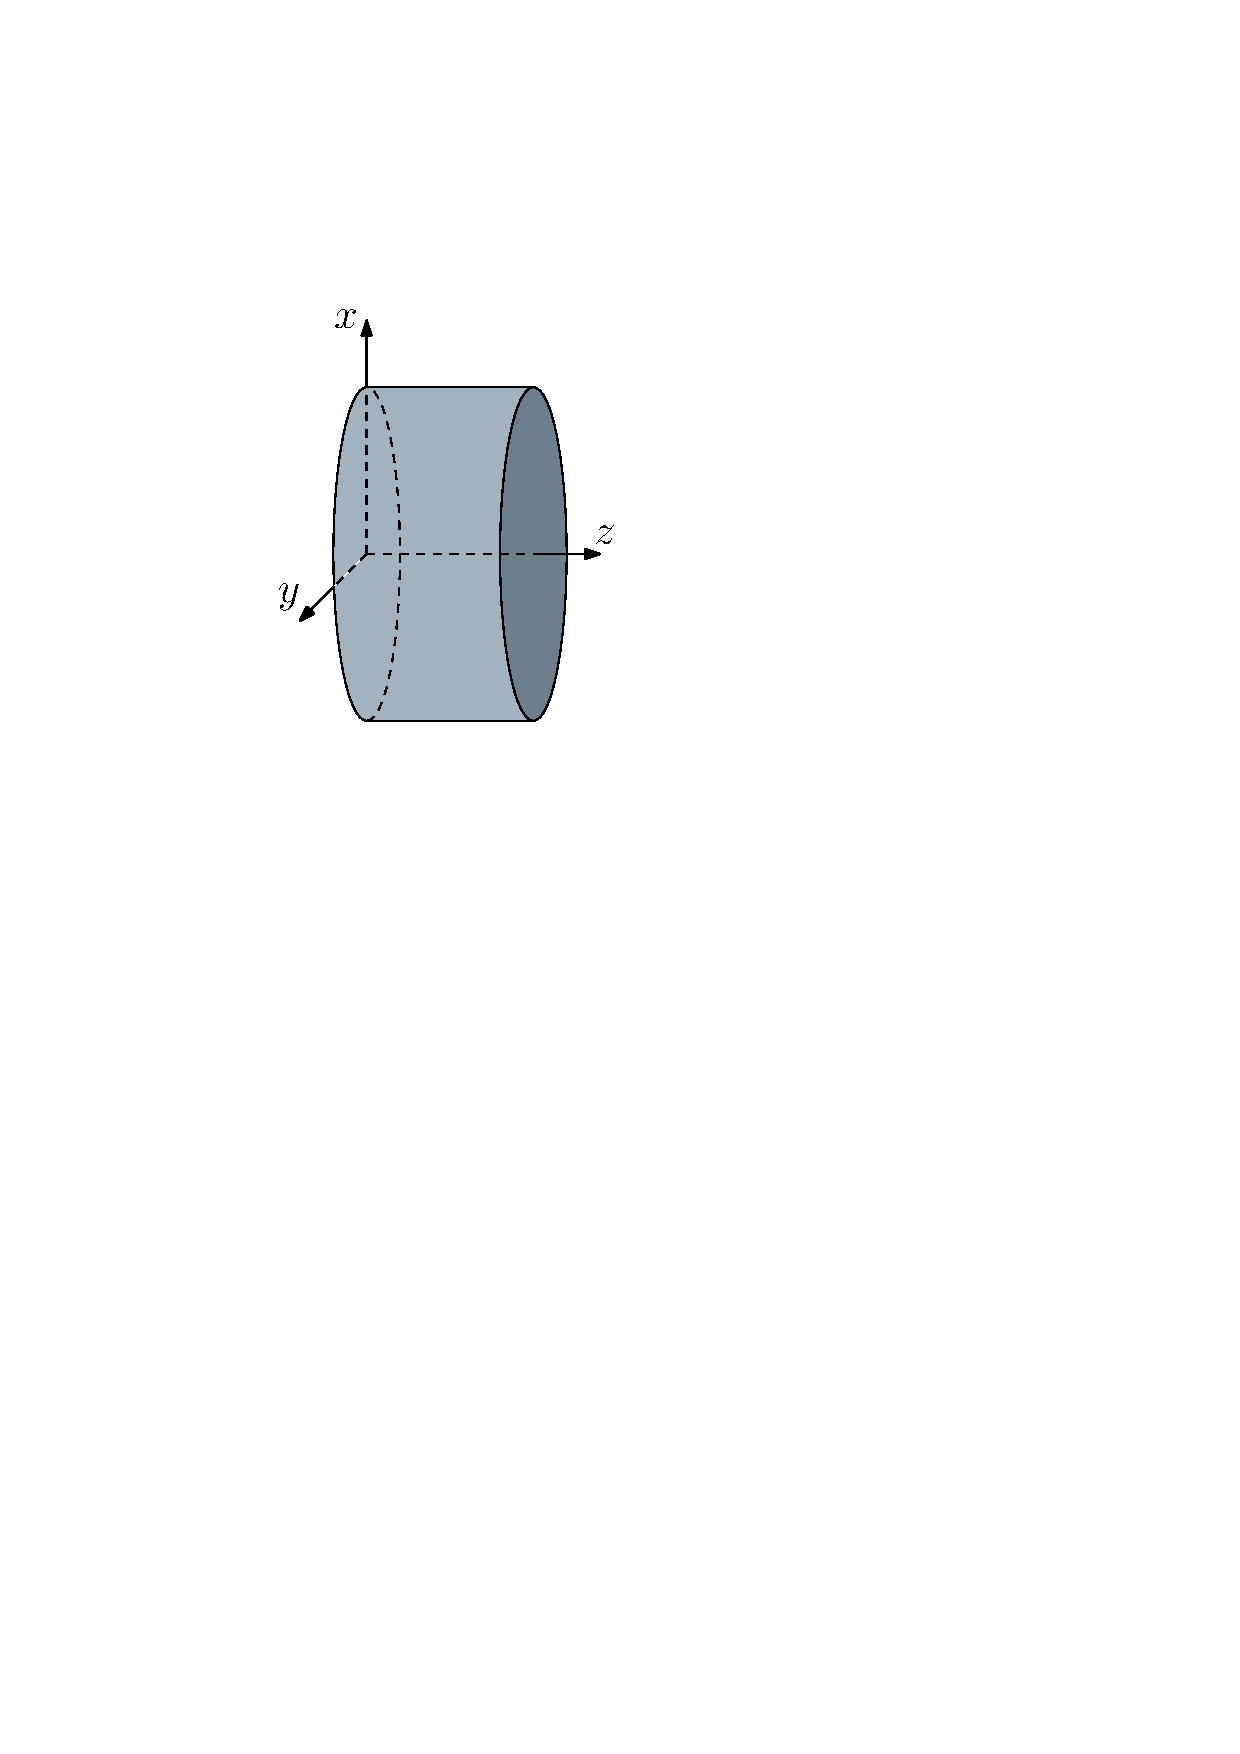
\includegraphics[scale=0.6]{./figures/pillbox.pdf}
	\end{columns}
	\vfill
	\begin{itemize}
		\item zylindersymmetrische Resonatormoden
		\begin{itemize}
			\setlength\itemsep{0.25em}
			\item TM und TE-Moden
			\item Bezeichnung durch drei Indizes $m, n, p$
		\end{itemize}
		
	\end{itemize}
\end{frame}

\begin{frame}[t]
	\begin{columns}[T]
		\column{0.5\textwidth}
		\begin{figure}[h]
			\centering
			\hspace*{0.70cm}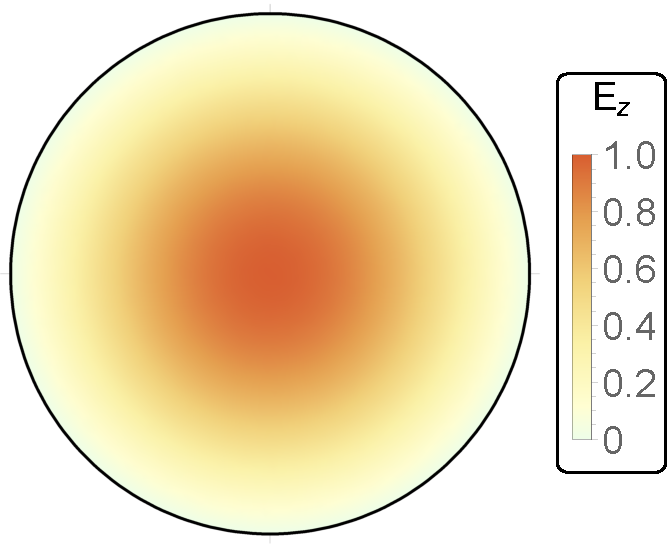
\includegraphics[scale=0.4]{./figures/tm010.pdf}
			\vspace*{-0.2cm}
			\caption{$\mathrm{TM}_{010}$}
		\end{figure}
		
		\column{0.5\textwidth}
		\begin{figure}[h]
			\centering
			\hspace*{0.70cm}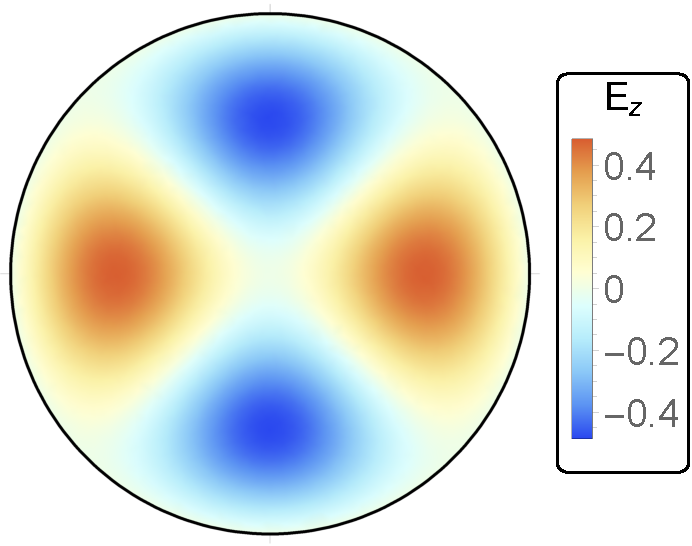
\includegraphics[scale=0.4]{./figures/tm210.pdf}
			\vspace*{-0.2cm}
			\caption{$\mathrm{TM}_{210}$}
		\end{figure}
	\end{columns}
	\vfill
	\begin{itemize}
		\item $\mathrm{TM}_{mnp}$ / $\mathrm{TE}_{mnp}$:
		\begin{itemize}
			\setlength\itemsep{0.25em}
			\item $m$: azimuthale Perioden
			\item $n$: radiale Knoten
			\item $p$: halbe longitudinale Perioden
		\end{itemize}
	\end{itemize}
\end{frame}


\subsection{elektrische Eigenschaften}
\begin{frame}{elektrische Eigenschaften von Hohlraumresonatoren}
	\begin{columns}[c]
		\column{0.6\textwidth}
		\begin{itemize}
			\item $RLC$-Parallelschwingkreis
			\begin{itemize}
				\item Eigenfrequenz $\omega_0$
				\item Kreisgüte $Q_0$
				\item Shuntimpedanz $R_\mathrm{S}$
			\end{itemize}
		\end{itemize}
		
		\column{0.4\textwidth}
		\centering
		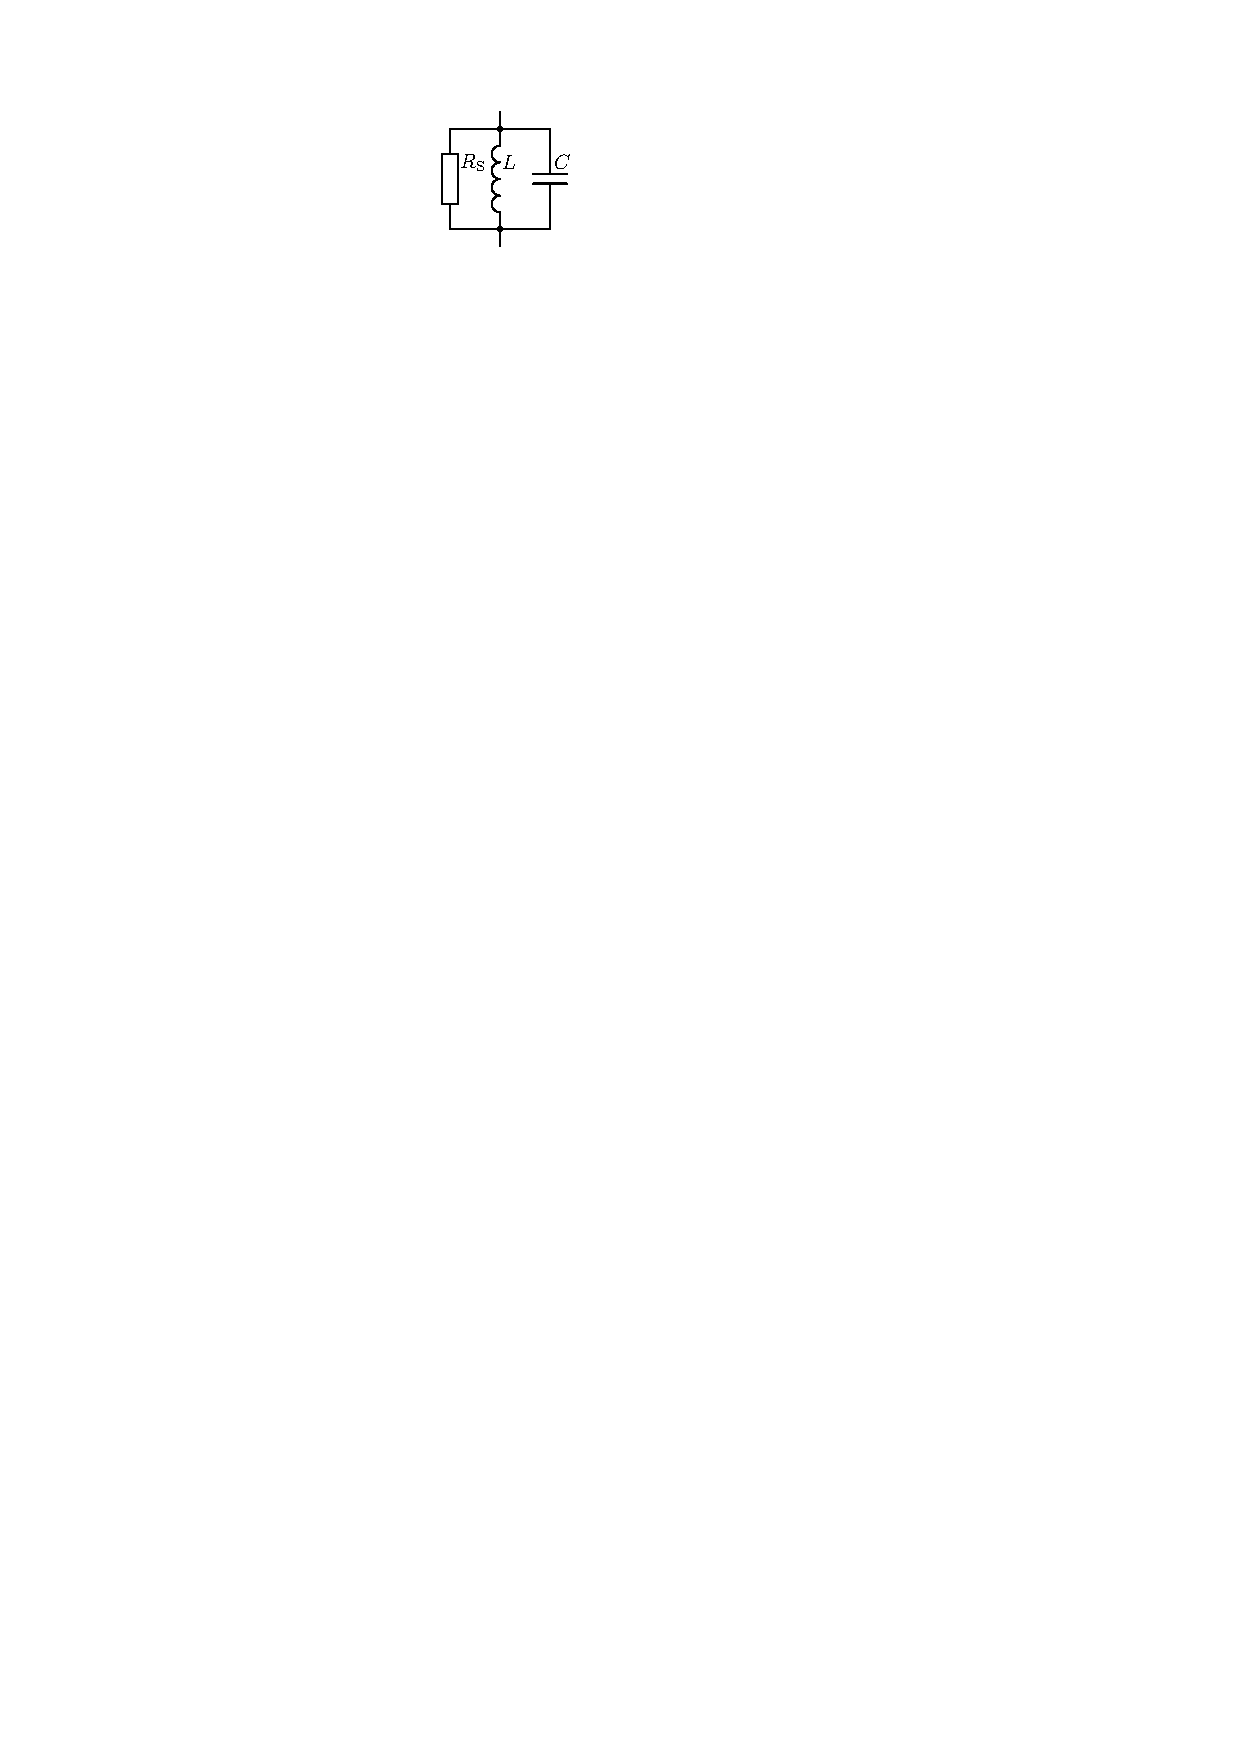
\includegraphics[width=0.6\textwidth]{./figures/RLC_circuit.pdf}
	\end{columns}
	
	\begin{itemize}
		\item Impedanzmodell:
		\begin{align*}
			Z(\omega) = \frac{R_\mathrm{S}}{1 + \mathrm{i} Q_0 \left( \frac{\omega}{\omega_0} - \frac{\omega_0}{\omega} \right)}
		\end{align*}
	\end{itemize}
\end{frame}

\begin{frame}{Kopplung}
	\begin{columns}[c]
		\column{0.65\textwidth}
		\begin{itemize}
			\item (induktive) Schleifenkopplung
		\end{itemize}
		
		\column{0.35\textwidth}
		\centering
		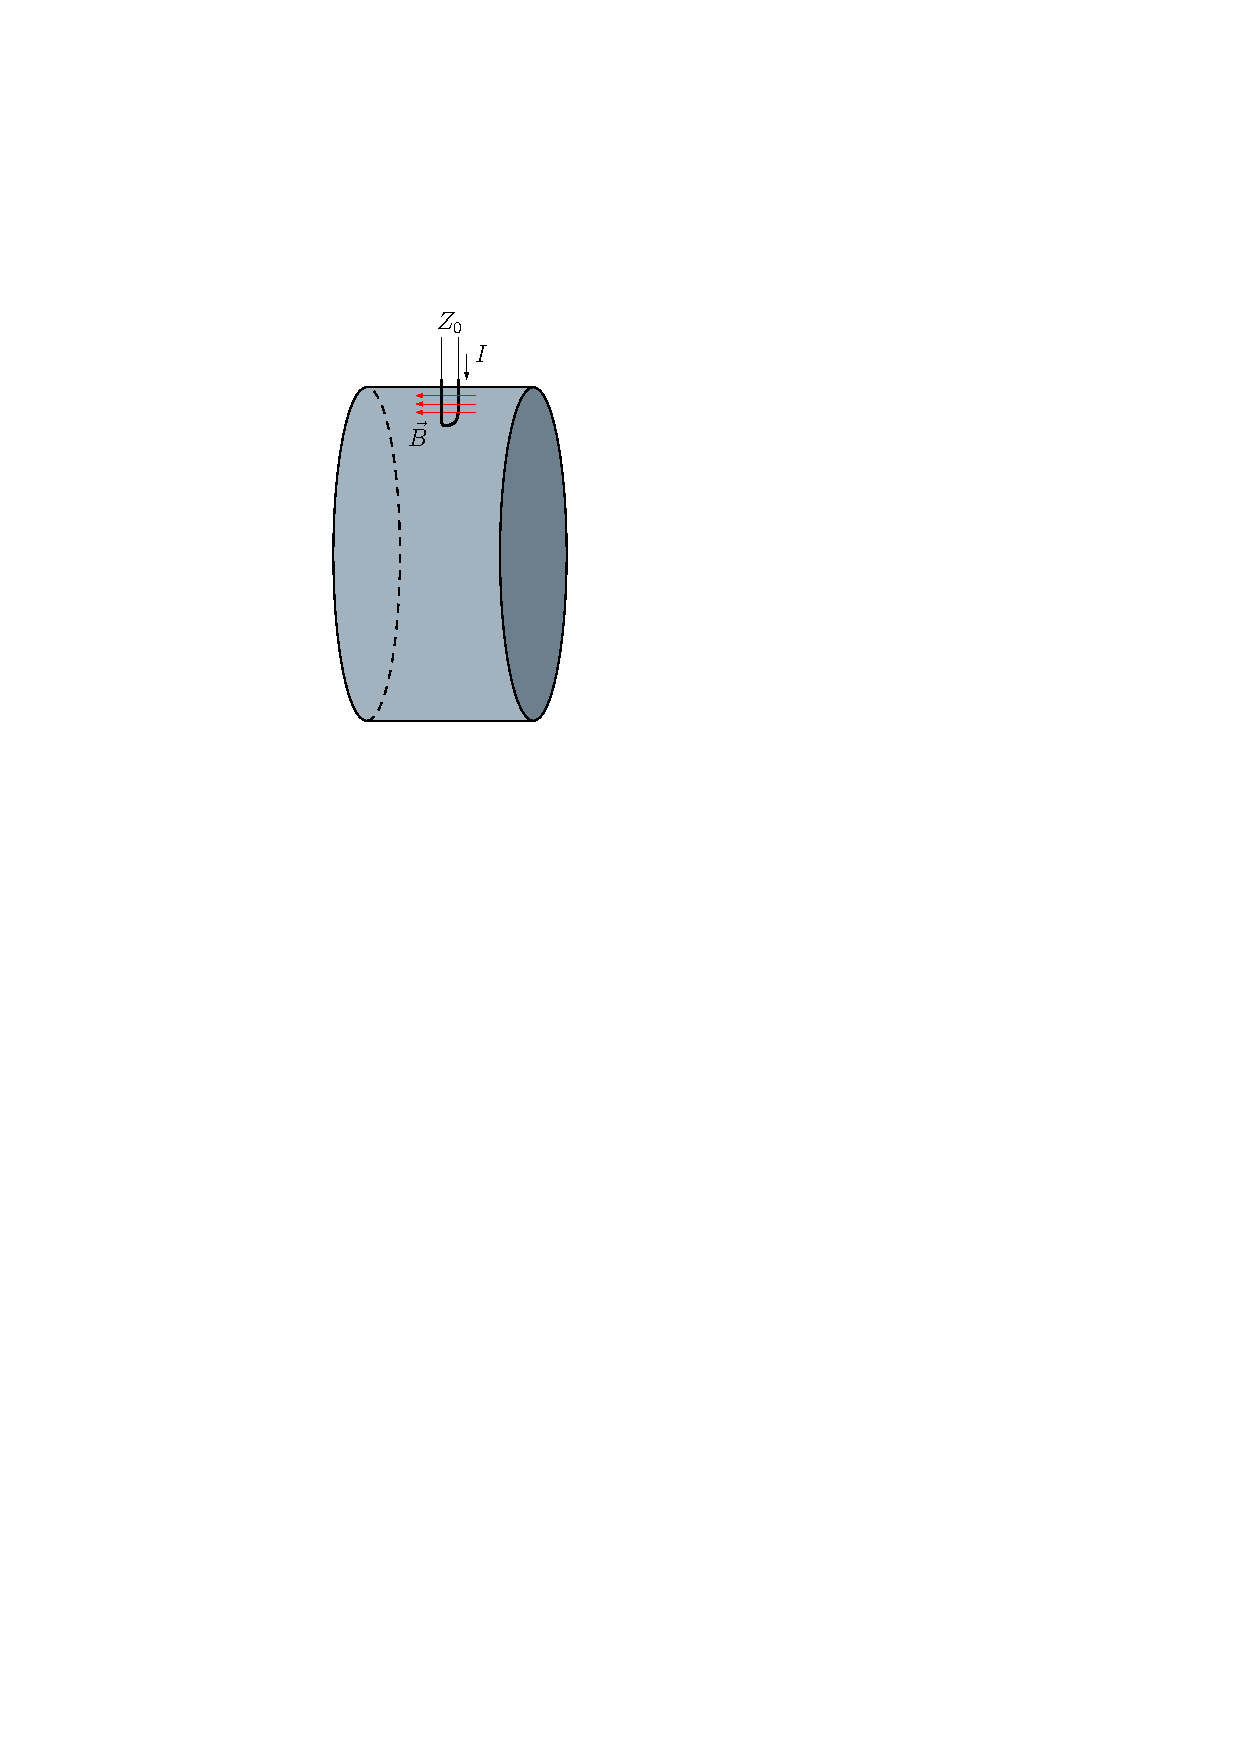
\includegraphics[scale=0.8]{./figures/pillbox_loop.pdf}
	\end{columns}
	
\end{frame}

\begin{frame}
	\begin{itemize}
		\item komplexer Reflexionsfaktor:
		\begin{align*}
			\rho(\omega) = \frac{(\kappa - 1) + \mathrm{i} Q_0 \left(\frac{\omega}{\omega_0} - \frac{\omega_0}{\omega}\right) }{(\kappa + 1) + \mathrm{i} Q_0 \left( \frac{\omega}{\omega_0} - \frac{\omega_0}{\omega} \right)}
		\end{align*}
	\end{itemize}
	
	Bild von Resonanzkurven (evtl. Phase?)
\end{frame}
	



\section{Resonante Störkörpermessung}

\begin{frame}{Störkörpermessung}
	\begin{itemize}
		\item Störung des Feldes durch dielektrische oder magnetische (Stör-)Körper (BILD?)
		\item Abhängig von Feldamplitude am Ort des Störkörpers
	\end{itemize}
\end{frame}

\begin{frame}{Resonante Störkörpermessung}
	\begin{itemize}
		\item Verschiebung der Resonanzfrequenz (kleine Störung):
		\begin{align*}
			\frac{\Delta \omega}{\omega_0} = \frac{\int_{V} \, \mathrm{d}V \left( \vec{E}_0^* \cdot \vec{P} + \vec{B}_0^* \cdot \vec{M} \right)}{4 W_0}
		\end{align*}
	
	\item Polarisation und Magnetisierung abhängig vom Körper (Material und Form)
	
	\item erlaubt die Bestimmung der Felder des ungestörten Resonators
	
	\end{itemize}
\end{frame}

\section{Störkörpermessungen}
\begin{frame}{Aufbau}
	\includegraphics[width=1.\textwidth]{./figures/messaufbau.pdf}
\end{frame}
\begin{frame}{Störkörpermessungen}
	\vspace*{2cm}
	\centering
	\begin{overpic}[width=0.95\textwidth,tics=10]{./figures/messaufbau_refpos.pdf}
		\put (45,20) {
				\fcolorbox{Black}{White}{% GNUPLOT: LaTeX picture with Postscript
\begingroup
  \makeatletter
  \providecommand\color[2][]{%
    \GenericError{(gnuplot) \space\space\space\@spaces}{%
      Package color not loaded in conjunction with
      terminal option `colourtext'%
    }{See the gnuplot documentation for explanation.%
    }{Either use 'blacktext' in gnuplot or load the package
      color.sty in LaTeX.}%
    \renewcommand\color[2][]{}%
  }%
  \providecommand\includegraphics[2][]{%
    \GenericError{(gnuplot) \space\space\space\@spaces}{%
      Package graphicx or graphics not loaded%
    }{See the gnuplot documentation for explanation.%
    }{The gnuplot epslatex terminal needs graphicx.sty or graphics.sty.}%
    \renewcommand\includegraphics[2][]{}%
  }%
  \providecommand\rotatebox[2]{#2}%
  \@ifundefined{ifGPcolor}{%
    \newif\ifGPcolor
    \GPcolortrue
  }{}%
  \@ifundefined{ifGPblacktext}{%
    \newif\ifGPblacktext
    \GPblacktexttrue
  }{}%
  % define a \g@addto@macro without @ in the name:
  \let\gplgaddtomacro\g@addto@macro
  % define empty templates for all commands taking text:
  \gdef\gplbacktext{}%
  \gdef\gplfronttext{}%
  \makeatother
  \ifGPblacktext
    % no textcolor at all
    \def\colorrgb#1{}%
    \def\colorgray#1{}%
  \else
    % gray or color?
    \ifGPcolor
      \def\colorrgb#1{\color[rgb]{#1}}%
      \def\colorgray#1{\color[gray]{#1}}%
      \expandafter\def\csname LTw\endcsname{\color{white}}%
      \expandafter\def\csname LTb\endcsname{\color{black}}%
      \expandafter\def\csname LTa\endcsname{\color{black}}%
      \expandafter\def\csname LT0\endcsname{\color[rgb]{1,0,0}}%
      \expandafter\def\csname LT1\endcsname{\color[rgb]{0,1,0}}%
      \expandafter\def\csname LT2\endcsname{\color[rgb]{0,0,1}}%
      \expandafter\def\csname LT3\endcsname{\color[rgb]{1,0,1}}%
      \expandafter\def\csname LT4\endcsname{\color[rgb]{0,1,1}}%
      \expandafter\def\csname LT5\endcsname{\color[rgb]{1,1,0}}%
      \expandafter\def\csname LT6\endcsname{\color[rgb]{0,0,0}}%
      \expandafter\def\csname LT7\endcsname{\color[rgb]{1,0.3,0}}%
      \expandafter\def\csname LT8\endcsname{\color[rgb]{0.5,0.5,0.5}}%
    \else
      % gray
      \def\colorrgb#1{\color{black}}%
      \def\colorgray#1{\color[gray]{#1}}%
      \expandafter\def\csname LTw\endcsname{\color{white}}%
      \expandafter\def\csname LTb\endcsname{\color{black}}%
      \expandafter\def\csname LTa\endcsname{\color{black}}%
      \expandafter\def\csname LT0\endcsname{\color{black}}%
      \expandafter\def\csname LT1\endcsname{\color{black}}%
      \expandafter\def\csname LT2\endcsname{\color{black}}%
      \expandafter\def\csname LT3\endcsname{\color{black}}%
      \expandafter\def\csname LT4\endcsname{\color{black}}%
      \expandafter\def\csname LT5\endcsname{\color{black}}%
      \expandafter\def\csname LT6\endcsname{\color{black}}%
      \expandafter\def\csname LT7\endcsname{\color{black}}%
      \expandafter\def\csname LT8\endcsname{\color{black}}%
    \fi
  \fi
    \setlength{\unitlength}{0.0500bp}%
    \ifx\gptboxheight\undefined%
      \newlength{\gptboxheight}%
      \newlength{\gptboxwidth}%
      \newsavebox{\gptboxtext}%
    \fi%
    \setlength{\fboxrule}{0.5pt}%
    \setlength{\fboxsep}{1pt}%
\begin{picture}(3400.00,2124.00)%
    \gplgaddtomacro\gplbacktext{%
    }%
    \gplgaddtomacro\gplfronttext{%
      \csname LTb\endcsname%
      \put(176,1116){\rotatebox{-270}{\makebox(0,0){\strut{}$|\rho|$}}}%
      \put(1699,154){\makebox(0,0){\strut{}$\omega$}}%
      \csname LTb\endcsname%
      \put(2091,285){\makebox(0,0){\strut{}\scriptsize{$\omega_0$}}}%
    }%
    \gplbacktext
    \put(0,0){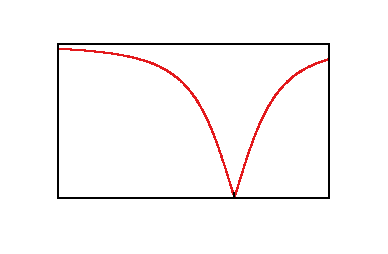
\includegraphics{./plots/resonanzkurve_ref}}%
    \gplfronttext
  \end{picture}%
\endgroup
}
			}
	\end{overpic}
\end{frame}

\begin{frame}{Störkörpermessungen}
	\addtocounter{framenumber}{-1} 
	\vspace*{2cm}
	\centering
	\begin{overpic}[width=0.95\textwidth,tics=10]{./figures/messaufbau_messpos.pdf}
		\put (45,20) {
			\fcolorbox{Black}{White}{% GNUPLOT: LaTeX picture with Postscript
\begingroup
  \makeatletter
  \providecommand\color[2][]{%
    \GenericError{(gnuplot) \space\space\space\@spaces}{%
      Package color not loaded in conjunction with
      terminal option `colourtext'%
    }{See the gnuplot documentation for explanation.%
    }{Either use 'blacktext' in gnuplot or load the package
      color.sty in LaTeX.}%
    \renewcommand\color[2][]{}%
  }%
  \providecommand\includegraphics[2][]{%
    \GenericError{(gnuplot) \space\space\space\@spaces}{%
      Package graphicx or graphics not loaded%
    }{See the gnuplot documentation for explanation.%
    }{The gnuplot epslatex terminal needs graphicx.sty or graphics.sty.}%
    \renewcommand\includegraphics[2][]{}%
  }%
  \providecommand\rotatebox[2]{#2}%
  \@ifundefined{ifGPcolor}{%
    \newif\ifGPcolor
    \GPcolortrue
  }{}%
  \@ifundefined{ifGPblacktext}{%
    \newif\ifGPblacktext
    \GPblacktexttrue
  }{}%
  % define a \g@addto@macro without @ in the name:
  \let\gplgaddtomacro\g@addto@macro
  % define empty templates for all commands taking text:
  \gdef\gplbacktext{}%
  \gdef\gplfronttext{}%
  \makeatother
  \ifGPblacktext
    % no textcolor at all
    \def\colorrgb#1{}%
    \def\colorgray#1{}%
  \else
    % gray or color?
    \ifGPcolor
      \def\colorrgb#1{\color[rgb]{#1}}%
      \def\colorgray#1{\color[gray]{#1}}%
      \expandafter\def\csname LTw\endcsname{\color{white}}%
      \expandafter\def\csname LTb\endcsname{\color{black}}%
      \expandafter\def\csname LTa\endcsname{\color{black}}%
      \expandafter\def\csname LT0\endcsname{\color[rgb]{1,0,0}}%
      \expandafter\def\csname LT1\endcsname{\color[rgb]{0,1,0}}%
      \expandafter\def\csname LT2\endcsname{\color[rgb]{0,0,1}}%
      \expandafter\def\csname LT3\endcsname{\color[rgb]{1,0,1}}%
      \expandafter\def\csname LT4\endcsname{\color[rgb]{0,1,1}}%
      \expandafter\def\csname LT5\endcsname{\color[rgb]{1,1,0}}%
      \expandafter\def\csname LT6\endcsname{\color[rgb]{0,0,0}}%
      \expandafter\def\csname LT7\endcsname{\color[rgb]{1,0.3,0}}%
      \expandafter\def\csname LT8\endcsname{\color[rgb]{0.5,0.5,0.5}}%
    \else
      % gray
      \def\colorrgb#1{\color{black}}%
      \def\colorgray#1{\color[gray]{#1}}%
      \expandafter\def\csname LTw\endcsname{\color{white}}%
      \expandafter\def\csname LTb\endcsname{\color{black}}%
      \expandafter\def\csname LTa\endcsname{\color{black}}%
      \expandafter\def\csname LT0\endcsname{\color{black}}%
      \expandafter\def\csname LT1\endcsname{\color{black}}%
      \expandafter\def\csname LT2\endcsname{\color{black}}%
      \expandafter\def\csname LT3\endcsname{\color{black}}%
      \expandafter\def\csname LT4\endcsname{\color{black}}%
      \expandafter\def\csname LT5\endcsname{\color{black}}%
      \expandafter\def\csname LT6\endcsname{\color{black}}%
      \expandafter\def\csname LT7\endcsname{\color{black}}%
      \expandafter\def\csname LT8\endcsname{\color{black}}%
    \fi
  \fi
    \setlength{\unitlength}{0.0500bp}%
    \ifx\gptboxheight\undefined%
      \newlength{\gptboxheight}%
      \newlength{\gptboxwidth}%
      \newsavebox{\gptboxtext}%
    \fi%
    \setlength{\fboxrule}{0.5pt}%
    \setlength{\fboxsep}{1pt}%
\begin{picture}(3400.00,2124.00)%
    \gplgaddtomacro\gplbacktext{%
    }%
    \gplgaddtomacro\gplfronttext{%
      \csname LTb\endcsname%
      \put(176,1116){\rotatebox{-270}{\makebox(0,0){\strut{}$|\rho|$}}}%
      \put(1699,154){\makebox(0,0){\strut{}$\omega$}}%
      \csname LTb\endcsname%
      \put(2091,285){\makebox(0,0){\strut{}\scriptsize{$\omega_0$}}}%
      \put(1700,775){\makebox(0,0){\strut{}$\Delta \omega$}}%
      \put(1308,285){\makebox(0,0){\strut{}\scriptsize{$\omega_1$}}}%
    }%
    \gplbacktext
    \put(0,0){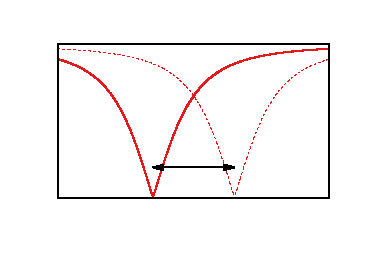
\includegraphics{./plots/resonanzkurve}}%
    \gplfronttext
  \end{picture}%
\endgroup
}
		}
	\end{overpic}
\end{frame}

\section{Ergebnisse}
\begin{frame}{Ergebnisse}
	Ergebnisse
\end{frame}

\begin{frame}{Literatur}
	\begin{thebibliography}{9}
		\bibitem{foot}
		Christopher J. Foot,
		\emph{Atomic Physics},
		Oxford University Press 2005
		
	\end{thebibliography}
	
\end{frame}

\beginbackup
% Hier die Backupfolien
\backupend

\end{document}